\chapter{КОМПОНЕНТНАЯ БАЗА}
\section{Введение}
В выборе компонентной базы мы будем руководствоваться следующими параметрами:
\begin{itemize}
\item простота интеграции;
\item дешевизна;
\item эргономичность.
\end{itemize}

\section{Микроконтроллер}
Если выбирать один контроллер,то он должен поддерживать протокол USB, SPI, иметь большое количество выводов, так как требуется задествовать много переферийных устройст, а кроме этого его частота должна быть достаточно высокой, чтобы поддерживать VGA интерфейс. На рынке есть процессор Atmel SAM3X8E ARM Cortex-M3 и плата на его базе(см. рис.\ref{fig:DueBoard}) с следующими характеристиками см. табл.\ref{tab:DueBoard}\cite{s_1}.
\begin{figure}[ht]
	\centering
     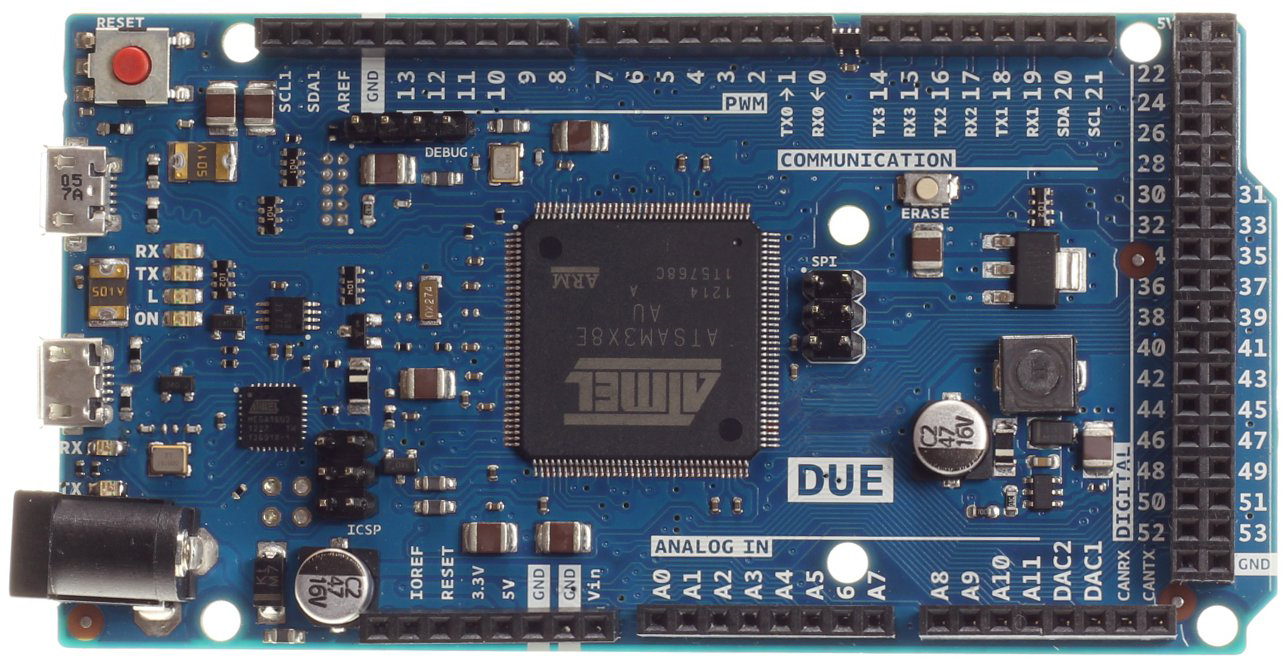
\includegraphics[scale=0.3]{due_board.jpg}
	\caption{Фотография платы.}
	\label{fig:DueBoard}
\end{figure}
\begin{table}
\centering
\begin{tabular}{|c|c|}
\hline 
Микроконтроллер & AT91SAM3X8E \\ 
\hline 
Рабочее напряжение & 3,3 В \\ 
\hline 
Входное напряжение (рекомендуемое) & 7-12 В \\ 
\hline 
Входное напряжение (предельное) & 6-20 В \\ 
\hline 
Цифровые Входы/Выходы & 54 \\ 
\hline 
Аналоговые входы & 12 \\ 
\hline 
Аналоговые выходы & 2 (ЦАП) \\ 
\hline 
Общий выходной постоянный ток & 50 мА \\ 
\hline 
Постоянный ток через вывод 3,3 В & 800 мА \\ 
\hline 
Постоянный ток через вывод 5 В & 800 мА \\ 
\hline 
Флеш-память & 512 КБ \\ 
\hline 
ОЗУ & 96 КБ(64 КБ и 32 КБ)\\ 
\hline 
Тактовая частота & 84 МГц \\ 
\hline 
\end{tabular} 
\caption{Характеристики платы.}
\label{tab:DueBoard}
\end{table}
На плате имеется 54 цифровых вход/выхода, 12 аналоговых входов, 4 UARTа (аппаратных последовательных порта), a генератор тактовой частоты 84 МГц, связь по USB с поддержкой OTG, 2 ЦАП (цифро-аналоговых преобразователя), 2 TWI, разъем питания,  разъем SPI, разъем JTAG, кнопка сброса и кнопка стирания. Так же 12 аналоговых входов, каждый из которых может обеспечить разрешение 12 бит (т.е. 4096 различных значений).
Отдельно надо заметим простоту интеграции c дисплеем посредством VGA видео интерфейса благодаря проекту ''DueVGA'' с открытым кодом на сайте распределённой системы управления версиями GitHub\cite{s_2}. Выберем этот контроллер для проекта.

\section{Привод}
Привод должен не только выполнять задачу передачи вращающего момента, то так же желательно, чтобы упростить модуль позиционирования тест-объекта, использовать привод с управляемым углом поворота. Наилучшим образом с этим справится шаговый двигатель, одной из ценных характеристик такого привода будет то, что его погрешность не будет расти при перемещении каретки на разные позиции. В последнее время шаговые двигатели приобрели особую популярность благодаря 3D принтерам, например 17HS8401(см. рис.\ref{fig:17hs8401_step_motor}).
\begin{figure}[ht]
	\centering
     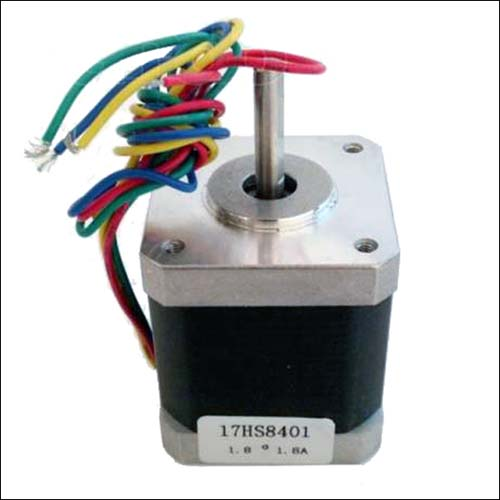
\includegraphics[scale=0.5]{17hs8401_step_motor.jpg}
	\caption{Фотография шагового двигателя.}
	\label{fig:17hs8401_step_motor}
\end{figure}
Для упрощения подключения шагового двигателя(далее двигателя) можно использовать драйвер двигателя и универсальный модуль для драйвера двигателя (см. рис.\ref{fig:Step_Motor_Driver}).
\begin{figure}[h]
    \centering
    \begin{subfigure}[b]{0.45\textwidth}
    \centering
        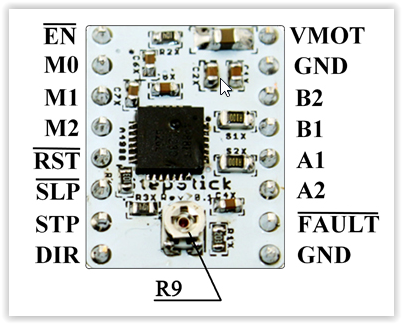
\includegraphics[scale=0.5]{Step_Motor_Driver.PNG}
        \caption{}
    \end{subfigure}
    \begin{subfigure}[b]{0.45\textwidth}
    \centering
        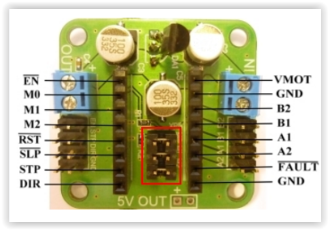
\includegraphics[scale=0.7]{Step_Motor_Driver_Uni_Model.PNG}
        \caption{}
    \end{subfigure}
    \caption{(а) Драйвер шагового двигателя;
    (б) Универсальный модуль подключения драйвера ш.д.}
    \label{fig:Step_Motor_Driver}
\end{figure}
Драйвер и модуль драйвера шагового двигателя содержат набор усилительных каскадов, которые под управлением драйвера подают напряжение в 12 вольт на вход двигателя, в тоже время сам драйвер управляется от импульсов напряжения 5 вольт и периодом не меньше 2 мкс, что очень удобно с точки зрение управления нашим центральным контроллером.

\section{Ограничители передвижения каретки}
Ограничители передвижения каретки или по другому концевики могут быть механическими, но мы остановимся на оптических(см. рис.\ref{fig:optical_end}). В их основе лежит оптрон tcst2103.
\begin{figure}[ht]
	\centering
     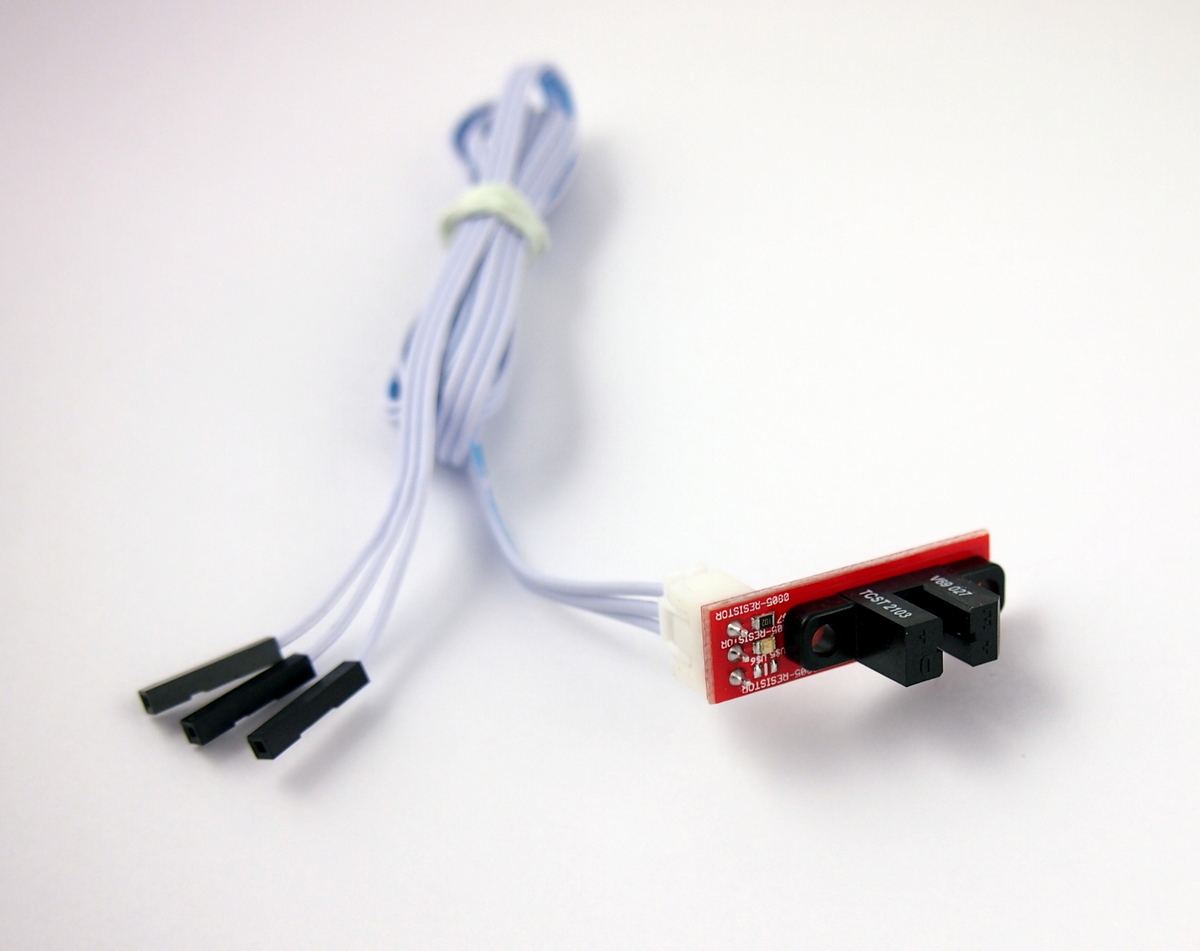
\includegraphics[scale=0.25]{optical_endswitch_with_cable_80cmP1240752.jpg}
	\caption{Оптический ограничитель передвижения каретки.}
	\label{fig:optical_end}
\end{figure}